\subsection{Geometry}
The $200$ kV geometry was derived from version one of the CST model. Some simplifications were made such that the geometry may be considered rotationally symmetric. The dimensions of the electrode, puck, puck elevator, vacuum chamber and insulator were derived from the model as depicted in fig.~\ref{fig:cst_geometry_yz}. The boundary conditions remained the same, except for the increase in voltage, when compared to the $60$ kV variant and the relative permittivity of the insulator was taken from the model to be $9.4$.

The geometry is depicted in fig.~\ref{fig:200kV_geometry_v1}. The numbers refer to the individual patches in the context of IGA. The patch boundaries are indicated by grey lines. The red lines represent homogeneous Dirichlet boundary conditions, the blue lines inhomogeneous Dirichlet boundary conditions with a value of $-200$ kV and the black lines indicate homogeneous Neumann boundaries.
The patches containing insulator material are colored in red and the blue patch indicates the part of the electrode boundary where the holes would be positioned.

The holes depicted in fig.~\ref{fig:cst_geometry_xz} are neglected in the current version of the model to obtain rotational symmetry for the geometry. However their volume will be taken into account later for the volume constraint.

We also observe triple points within the computational domain. These are defined by material boundaries between air/vacuum, steel and the insulator.

\begin{center}
\begin{figure}[H]
   \begin{subfigure}{0.45\textwidth}
      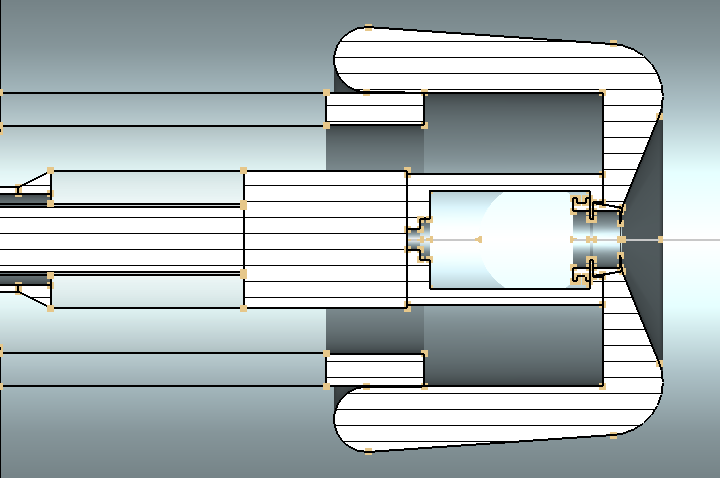
\includegraphics[width=\textwidth]{figures/200kV/png/v1_cutx}
      \caption{$y$-$z$ view for $x=0$.}
      \label{fig:cst_geometry_yz}
   \end{subfigure}
   \begin{subfigure}{0.45\textwidth}
      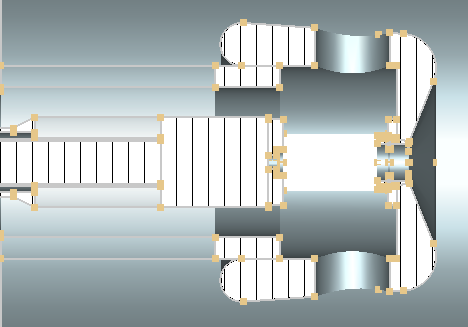
\includegraphics[width=\textwidth]{figures/200kV/png/v1_cuty}
      \caption{$x$-$z$ view for $y=0$.}
      \label{fig:cst_geometry_xz}
   \end{subfigure}
   \caption{CST model.}
\end{figure}
\end{center}

\begin{center}
\begin{figure}[H]
  \begin{tikzpicture}
\begin{axis}[
   scale only axis = true,
   width = 0.9\textwidth,
  axis equal,
  try min ticks=4,
  max space between ticks=1000pt,
  enlargelimits=true,
  colormap/Greens,
  point meta min = 0,
  point meta max = 2,
  x unit=m,
  y unit=m]

  \addplot[surf, shader=interp] table[point meta=\thisrow{c}]{figures/200kV/geometry/v1/geometry1.dat};

  \addplot[surf, shader=interp] table[point meta=\thisrow{c}]{figures/200kV/geometry/v1/geometry2.dat};

  \addplot[surf, shader=interp] table[point meta=\thisrow{c}]{figures/200kV/geometry/v1/geometry3.dat};

  \addplot[surf, shader=interp] table[point meta=\thisrow{c}]{figures/200kV/geometry/v1/geometry4.dat};

  \addplot[surf, shader=interp] table[point meta=\thisrow{c}]{figures/200kV/geometry/v1/geometry5.dat};

  \addplot[surf, shader=interp] table[point meta=\thisrow{c}]{figures/200kV/geometry/v1/geometry6.dat};

  \addplot[surf, shader=interp] table[point meta=\thisrow{c}]{figures/200kV/geometry/v1/geometry7.dat};

  \addplot[surf, shader=interp, colormap/Blues, point meta min = 0, point meta max = 1] table[point meta=\thisrow{c}]{figures/200kV/geometry/v1/geometry8.dat};

  \addplot[surf, shader=interp] table[point meta=\thisrow{c}]{figures/200kV/geometry/v1/geometry9.dat};

  \addplot[surf, shader=interp] table[point meta=\thisrow{c}]{figures/200kV/geometry/v1/geometry10.dat};

  \addplot[surf, shader=interp] table[point meta=\thisrow{c}]{figures/200kV/geometry/v1/geometry11.dat};

  \addplot[surf, shader=interp] table[point meta=\thisrow{c}]{figures/200kV/geometry/v1/geometry12.dat};

  \addplot[surf, shader=interp] table[point meta=\thisrow{c}]{figures/200kV/geometry/v1/geometry13.dat};

  \addplot[surf, shader=interp] table[point meta=\thisrow{c}]{figures/200kV/geometry/v1/geometry13.dat};

  \addplot[surf, shader=interp, colormap/Reds, point meta min = 0, point meta max = 1] table[point meta=\thisrow{c}]{figures/200kV/geometry/v1/geometry14.dat};

  \addplot[surf, shader=interp] table[point meta=\thisrow{c}]{figures/200kV/geometry/v1/geometry15.dat};

  \addplot[surf, shader=interp] table[point meta=\thisrow{c}]{figures/200kV/geometry/v1/geometry16.dat};

  \addplot[surf, shader=interp] table[point meta=\thisrow{c}]{figures/200kV/geometry/v1/geometry17.dat};

  \addplot[surf, shader=interp, colormap/Reds, point meta min = 0, point meta max = 1] table[point meta=\thisrow{c}]{figures/200kV/geometry/v1/geometry18.dat};

  \addplot[surf, shader=interp, colormap/Reds, point meta min = 0, point meta max = 1] table[point meta=\thisrow{c}]{figures/200kV/geometry/v1/geometry19.dat};

  \addplot[surf, shader=interp] table[point meta=\thisrow{c}]{figures/200kV/geometry/v1/geometry20.dat};

  \addplot[surf, shader=interp] table[point meta=\thisrow{c}]{figures/200kV/geometry/v1/geometry21.dat};

  \addplot[surf, shader=interp] table[point meta=\thisrow{c}]{figures/200kV/geometry/v1/geometry22.dat};

  \addplot[surf, shader=interp] table[point meta=\thisrow{c}]{figures/200kV/geometry/v1/geometry23.dat};

  \addplot[surf, shader=interp] table[point meta=\thisrow{c}]{figures/200kV/geometry/v1/geometry24.dat};

  % add patch indices
  \addplot[only marks, point meta=explicit symbolic, color=black, nodes near coords] coordinates{
  (0.28,-0.01) [(1)]
  (0.28,-0.005) [(2)]
  (0.28,0.005) [(3)]
  (0.28,0.015) [(4)]
  (0.28,0.045) [(5)]
  (0.24,0.075) [(6)]
  (0.185,0.075) [(7)]
  (0.165,0.075) [(8)]
  (0.125,0.075) [(9)]
  (0.095,0.065) [(10)]
  (0.1,0.04) [(11)]
  (0.05,0.075) [(12)]
  (0.06,0.045) [(13)]
  (0.05,0.03) [(14)]
  (0.03,0.02) [(15)]
  (0.07,0.017) [(16)]
  (0.005,0.01) [(17)]
  (0.055,0.007) [(18)]
  (0.007,0.004) [(19)]
  (0.035,-0.005) [(20)]
  (0.11,0.017) [(21)]
  (0.17,0.01) [(22)]
  (0.135,0.0175) [(23)]
  (0.165,0.0275) [(24)]
  };

  % add patch boundaries
  \addplot[color=brewerblue] table{figures/200kV/boundary/v1/boundaries11.dat};
  \addplot[color=brewerred] table{figures/200kV/boundary/v1/boundaries12.dat};
  \addplot[color=black] table{figures/200kV/boundary/v1/boundaries13.dat};
  \addplot[color=brewergrey] table{figures/200kV/boundary/v1/boundaries14.dat};

  \addplot[color=brewerblue] table{figures/200kV/boundary/v1/boundaries21.dat};
  \addplot[color=brewerred] table{figures/200kV/boundary/v1/boundaries22.dat};
  \addplot[color=brewergrey] table{figures/200kV/boundary/v1/boundaries23.dat};
  \addplot[color=brewergrey] table{figures/200kV/boundary/v1/boundaries24.dat};

  \addplot[color=brewerblue] table{figures/200kV/boundary/v1/boundaries31.dat};
  \addplot[color=brewerred] table{figures/200kV/boundary/v1/boundaries32.dat};
  \addplot[color=brewergrey] table{figures/200kV/boundary/v1/boundaries33.dat};
  \addplot[color=brewergrey] table{figures/200kV/boundary/v1/boundaries34.dat};

  \addplot[color=brewerblue] table{figures/200kV/boundary/v1/boundaries41.dat};
  \addplot[color=brewerred] table{figures/200kV/boundary/v1/boundaries42.dat};
  \addplot[color=brewergrey] table{figures/200kV/boundary/v1/boundaries43.dat};
  \addplot[color=brewergrey] table{figures/200kV/boundary/v1/boundaries44.dat};

  \addplot[color=brewerblue] table{figures/200kV/boundary/v1/boundaries51.dat};
  \addplot[color=brewerred] table{figures/200kV/boundary/v1/boundaries52.dat};
  \addplot[color=brewergrey] table{figures/200kV/boundary/v1/boundaries53.dat};
  \addplot[color=brewergrey] table{figures/200kV/boundary/v1/boundaries54.dat};

  \addplot[color=brewergrey] table{figures/200kV/boundary/v1/boundaries61.dat};
  \addplot[color=brewergrey] table{figures/200kV/boundary/v1/boundaries62.dat};
  \addplot[color=brewerblue] table{figures/200kV/boundary/v1/boundaries63.dat};
  \addplot[color=brewerred] table{figures/200kV/boundary/v1/boundaries64.dat};

  \addplot[color=brewergrey] table{figures/200kV/boundary/v1/boundaries71.dat};
  \addplot[color=brewergrey] table{figures/200kV/boundary/v1/boundaries72.dat};
  \addplot[color=brewerblue] table{figures/200kV/boundary/v1/boundaries73.dat};
  \addplot[color=brewerred] table{figures/200kV/boundary/v1/boundaries74.dat};

  \addplot[color=brewergrey] table{figures/200kV/boundary/v1/boundaries81.dat};
  \addplot[color=brewergrey] table{figures/200kV/boundary/v1/boundaries82.dat};
  \addplot[color=brewerblue] table{figures/200kV/boundary/v1/boundaries83.dat};
  \addplot[color=brewerred] table{figures/200kV/boundary/v1/boundaries84.dat};

  \addplot[color=brewergrey] table{figures/200kV/boundary/v1/boundaries91.dat};
  \addplot[color=brewergrey] table{figures/200kV/boundary/v1/boundaries92.dat};
  \addplot[color=brewerblue] table{figures/200kV/boundary/v1/boundaries93.dat};
  \addplot[color=brewerred] table{figures/200kV/boundary/v1/boundaries94.dat};

  \addplot[color=brewergrey] table{figures/200kV/boundary/v1/boundaries101.dat};
  \addplot[color=brewerblue] table{figures/200kV/boundary/v1/boundaries102.dat};
  \addplot[color=brewergrey] table{figures/200kV/boundary/v1/boundaries103.dat};
  \addplot[color=brewergrey] table{figures/200kV/boundary/v1/boundaries104.dat};

  \addplot[color=brewergrey] table{figures/200kV/boundary/v1/boundaries111.dat};
  \addplot[color=brewerblue] table{figures/200kV/boundary/v1/boundaries112.dat};
  \addplot[color=brewerblue] table{figures/200kV/boundary/v1/boundaries113.dat};
  \addplot[color=brewergrey] table{figures/200kV/boundary/v1/boundaries114.dat};

  \addplot[color=brewerred] table{figures/200kV/boundary/v1/boundaries121.dat};
  \addplot[color=brewergrey] table{figures/200kV/boundary/v1/boundaries122.dat};
  \addplot[color=brewergrey] table{figures/200kV/boundary/v1/boundaries123.dat};
  \addplot[color=brewerred] table{figures/200kV/boundary/v1/boundaries124.dat};

  \addplot[color=brewerred] table{figures/200kV/boundary/v1/boundaries131.dat};
  \addplot[color=brewergrey] table{figures/200kV/boundary/v1/boundaries132.dat};
  \addplot[color=brewergrey] table{figures/200kV/boundary/v1/boundaries133.dat};
  \addplot[color=brewergrey] table{figures/200kV/boundary/v1/boundaries134.dat};

  \addplot[color=brewerred] table{figures/200kV/boundary/v1/boundaries141.dat};
  \addplot[color=brewerblue] table{figures/200kV/boundary/v1/boundaries142.dat};
  \addplot[color=brewergrey] table{figures/200kV/boundary/v1/boundaries143.dat};
  \addplot[color=brewergrey] table{figures/200kV/boundary/v1/boundaries144.dat};

  \addplot[color=brewerred] table{figures/200kV/boundary/v1/boundaries151.dat};
  \addplot[color=brewergrey] table{figures/200kV/boundary/v1/boundaries152.dat};
  \addplot[color=brewergrey] table{figures/200kV/boundary/v1/boundaries153.dat};
  \addplot[color=brewergrey] table{figures/200kV/boundary/v1/boundaries154.dat};

  \addplot[color=brewergrey] table{figures/200kV/boundary/v1/boundaries161.dat};
  \addplot[color=brewergrey] table{figures/200kV/boundary/v1/boundaries162.dat};
  \addplot[color=brewergrey] table{figures/200kV/boundary/v1/boundaries163.dat};
  \addplot[color=brewerblue] table{figures/200kV/boundary/v1/boundaries164.dat};

  \addplot[color=brewerred] table{figures/200kV/boundary/v1/boundaries171.dat};
  \addplot[color=brewergrey] table{figures/200kV/boundary/v1/boundaries172.dat};
  \addplot[color=brewergrey] table{figures/200kV/boundary/v1/boundaries173.dat};
  \addplot[color=brewergrey] table{figures/200kV/boundary/v1/boundaries174.dat};

  \addplot[color=brewergrey] table{figures/200kV/boundary/v1/boundaries181.dat};
  \addplot[color=brewerblue] table{figures/200kV/boundary/v1/boundaries182.dat};
  \addplot[color=brewergrey] table{figures/200kV/boundary/v1/boundaries183.dat};
  \addplot[color=brewergrey] table{figures/200kV/boundary/v1/boundaries184.dat};

  \addplot[color=brewerred] table{figures/200kV/boundary/v1/boundaries191.dat};
  \addplot[color=brewergrey] table{figures/200kV/boundary/v1/boundaries192.dat};
  \addplot[color=brewergrey] table{figures/200kV/boundary/v1/boundaries193.dat};
  \addplot[color=brewergrey] table{figures/200kV/boundary/v1/boundaries194.dat};

  \addplot[color=brewerred] table{figures/200kV/boundary/v1/boundaries201.dat};
  \addplot[color=brewerblue] table{figures/200kV/boundary/v1/boundaries202.dat};
  \addplot[color=black] table{figures/200kV/boundary/v1/boundaries203.dat};
  \addplot[color=brewergrey] table{figures/200kV/boundary/v1/boundaries204.dat};

  \addplot[color=brewergrey] table{figures/200kV/boundary/v1/boundaries211.dat};
  \addplot[color=brewergrey] table{figures/200kV/boundary/v1/boundaries212.dat};
  \addplot[color=brewerblue] table{figures/200kV/boundary/v1/boundaries213.dat};
  \addplot[color=brewerblue] table{figures/200kV/boundary/v1/boundaries214.dat};

  \addplot[color=brewerblue] table{figures/200kV/boundary/v1/boundaries221.dat};
  \addplot[color=brewerblue] table{figures/200kV/boundary/v1/boundaries222.dat};
  \addplot[color=brewerblue] table{figures/200kV/boundary/v1/boundaries223.dat};
  \addplot[color=brewergrey] table{figures/200kV/boundary/v1/boundaries224.dat};

  \addplot[color=brewergrey] table{figures/200kV/boundary/v1/boundaries231.dat};
  \addplot[color=brewerblue] table{figures/200kV/boundary/v1/boundaries232.dat};
  \addplot[color=brewergrey] table{figures/200kV/boundary/v1/boundaries233.dat};
  \addplot[color=brewergrey] table{figures/200kV/boundary/v1/boundaries234.dat};

  \addplot[color=brewerblue] table{figures/200kV/boundary/v1/boundaries241.dat};
  \addplot[color=brewerblue] table{figures/200kV/boundary/v1/boundaries242.dat};
  \addplot[color=brewergrey] table{figures/200kV/boundary/v1/boundaries243.dat};
  \addplot[color=brewerblue] table{figures/200kV/boundary/v1/boundaries244.dat};

\end{axis}
\end{tikzpicture}

  \caption{200 kV Photocathode geometry and boundary conditions.}
  \label{fig:200kV_geometry_v1}
\end{figure}
\end{center}

\subsection{Electric Field}
The solution for the electric field is shown in fig.~\ref{fig:200kV_electric_field}.
It was computed with $p=3$ as the degree of the basis functions and $n_\mathrm{sub}=16$ as the number of elements that each knot vector is uniformly split into. The fairly low number of subdomains was chosen to improve performance in regards to the optimization.
It is evident that there exist parts of the domain where the magnitude of the electric field is close to the limit of $10 \frac{\mathrm{MV}}{\mathrm{m}}$. There are also very high gradients visible at the triple points, however these also coincide with sharp corners so numerical issues might play a role.

\begin{center}
\begin{figure}[H]
  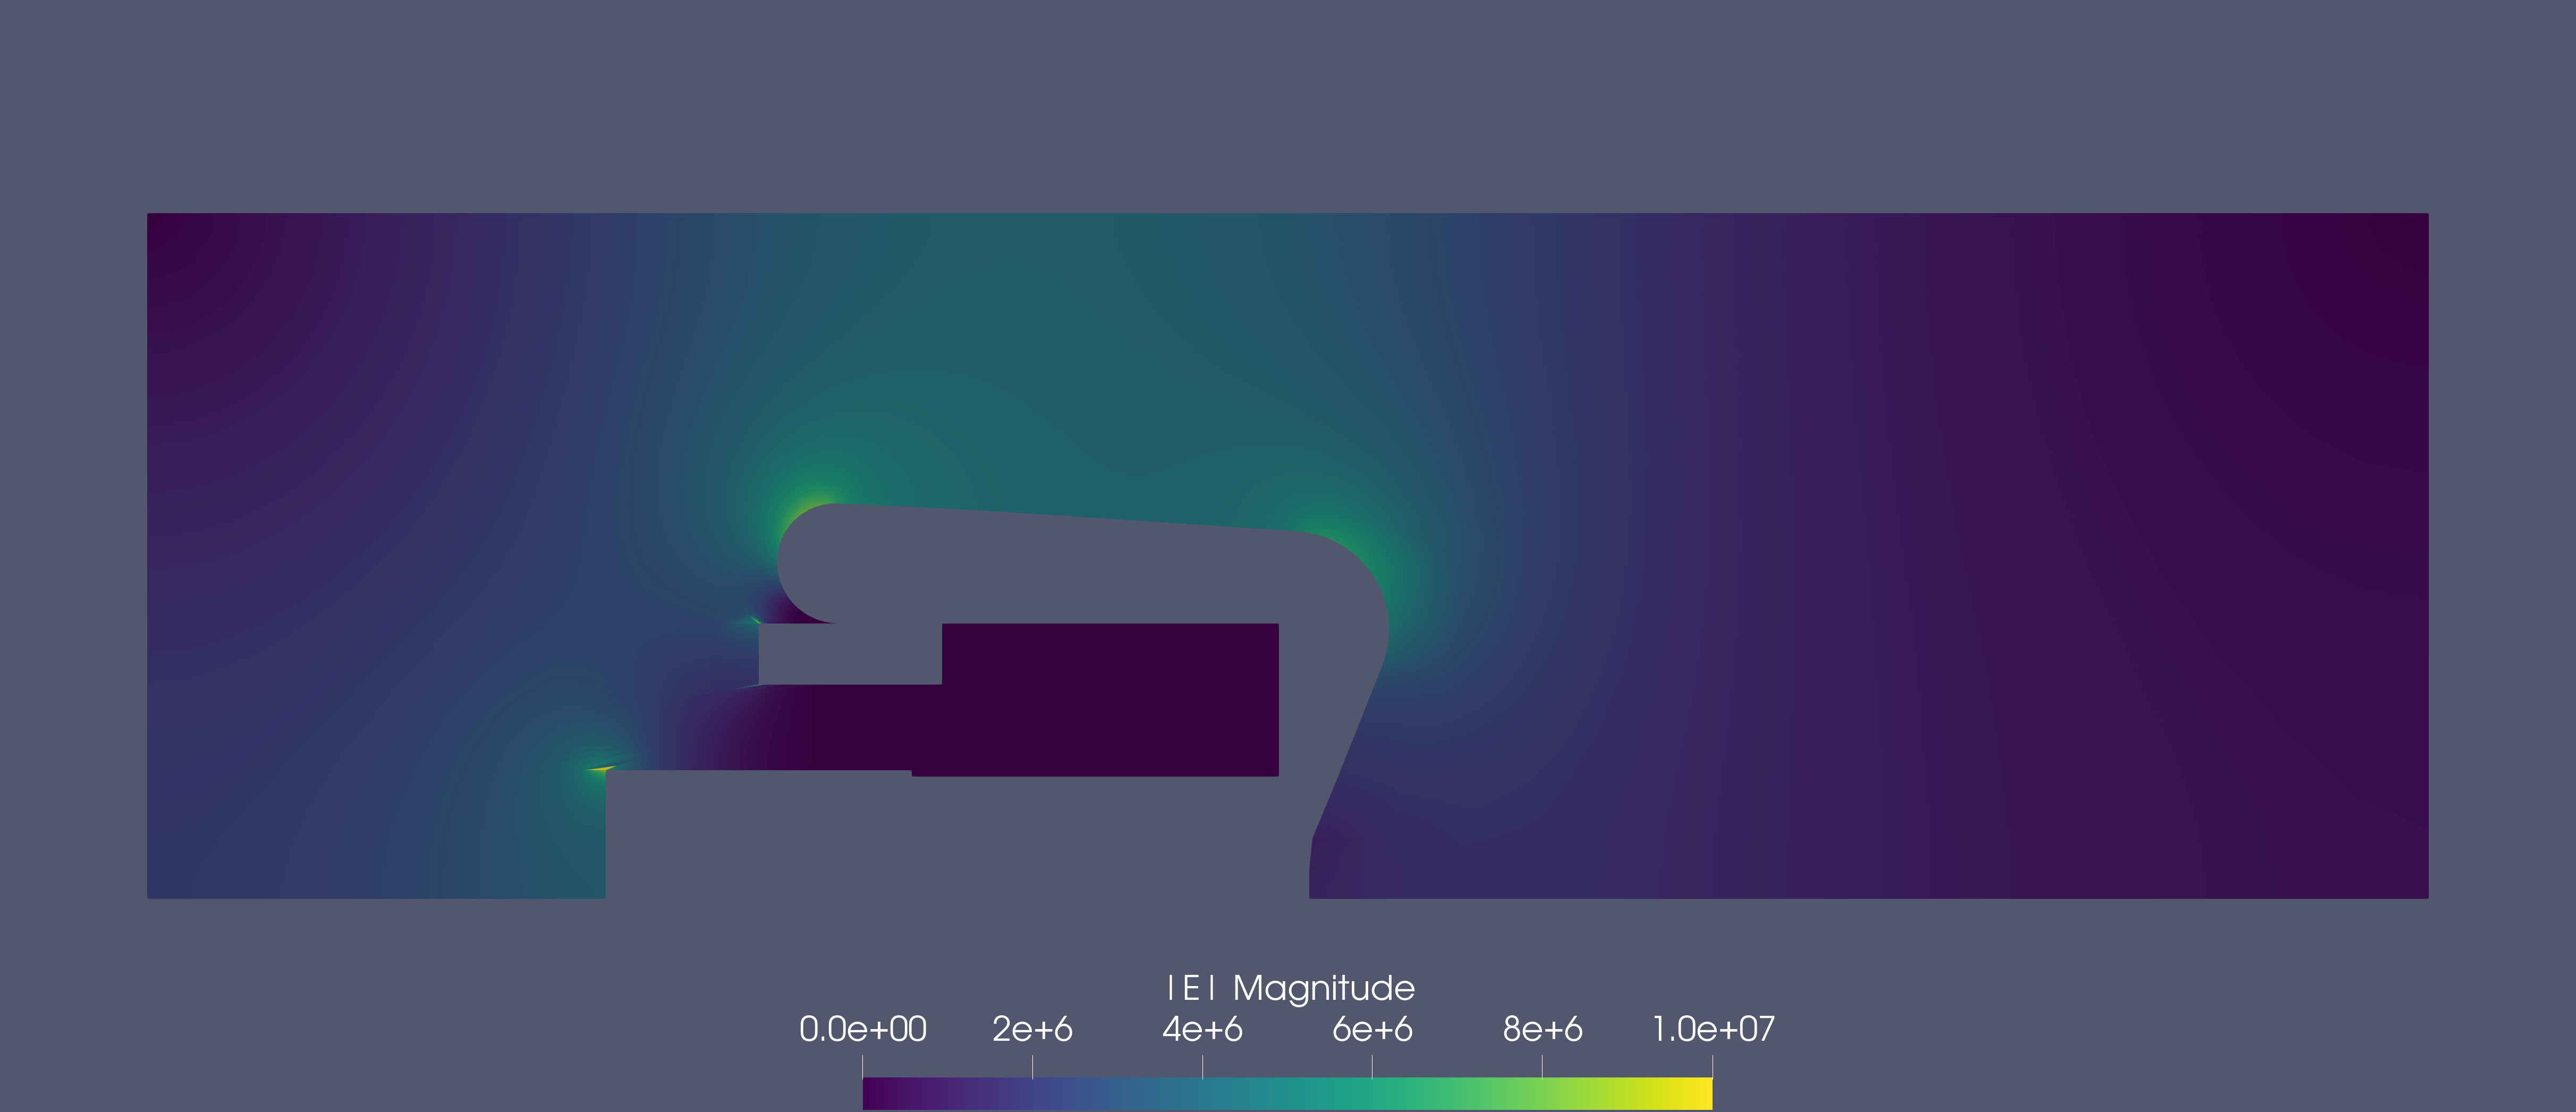
\includegraphics[width=\textwidth]{figures/200kV/png/order=3}
  \caption{Absolute value of the electric field with $p=3$ and $n_\mathrm{sub}=16$.}
  \label{fig:200kV_electric_field}
\end{figure}
\end{center}

\subsection{Optimization}
The aim of the optimization is to minimize the maximal field amplitudes. For practicality we will only look at the critical points of the geometry, i.~e.~the curvatures of the outer electrode and the triple points. The lower part of the geometry will remain fixed so only the electrode boundaries of patches 5 through 11 from fig.~\ref{fig:200kV_geometry_v1} and their respective control points are the DoFs. Aside from the fixed part of the geometry we also consider a volume constraint.

\subsubsection{Volume Constraint}
One of the constraints for the optimization is the weight of the electrode and thus its volume.
We first compute the volume of the patches by taking into account the rotational symmetry and discretizing $V_{\mathrm{ptc}} = \int_V r\, \drm r\, \drm \varphi\, \drm z$ via numerical quadrature. We can then obtain the volume of the electrode by subtracting $V_{\mathrm{ptc}}$ from the cylinder formed by the vacuumchamber.
We still need to consider the holes inside the electrode, visible in \ref{fig:cst_geometry_xz}. Their volume is computed by considering a cylinder with its height as a function of $z$. The curvature in $x$ and $y$ is disregarded, since it is the same for both coordinates. We can therefore determine the value by discretizing $V_{h} = \int_V \drm x\, \drm y\, \drm z$.
Lastly the connection of the electrode with the insulator as well as the lift and the connection to the cable are not part of the electrode and thus their volume is subtracted as well.
In total the physical constraint is set at $625\ \mathrm{cm}^3$ and the volume of the current geometry is computed as approximately $608\ \mathrm{cm}^3$.

\subsubsection{Cost Function}
For the cost function we first define $E_i$ as the maximal absolute electric field across the quadrature nodes of patch $i$.
We then define the cost function to be
\begin{align}
   c = \frac{1}{|I|} \sum_{i \in I} E_i
\end{align}
where $I$ contains the indices of the patches of interest.

\subsubsection{Additional Constraints}
As an additional constraint we require $C^1$ continuity of the section that is optimized. The starting nurbs is depicted in fig.~\ref{fig:nurbs}. Furthermore the control points, which represent the DoFs, are constrained to stay inside their respective patch boundaries and in the correct order. To correctly model the holes with patch 8 the adjacent control points are constrained to only move vertically.

\begin{center}
\begin{figure}[H]
  \begin{tikzpicture}
\begin{axis}[
   scale only axis = true,
   width = 0.45\textwidth,
   axis equal,
   try min ticks=4,
   max space between ticks=1000pt,
   enlargelimits=true,
   x unit=m,
   y unit=m]

   \addplot[color=brewergrey] table {figures/200kV/nurbs/nurbs_5_1.dat};
   \addplot[color=brewerred, mark=*] table {figures/200kV/nurbs/nurbs_5_1_coefs.dat};
   \addplot[color=brewergrey, dashed] table {figures/200kV/nurbs/nurbs_5_1_net.dat};

   \addplot[color=brewergrey] table {figures/200kV/nurbs/nurbs_6_3.dat};
   \addplot[color=brewerred, mark=*] table {figures/200kV/nurbs/nurbs_6_3_coefs.dat};
   \addplot[color=brewergrey, dashed] table {figures/200kV/nurbs/nurbs_6_3_net.dat};

   \addplot[color=brewergrey] table {figures/200kV/nurbs/nurbs_7_3.dat};
   \addplot[color=brewerred, mark=*] table {figures/200kV/nurbs/nurbs_7_3_coefs.dat};
   \addplot[color=brewergrey, dashed] table {figures/200kV/nurbs/nurbs_7_3_net.dat};

   \addplot[color=brewergrey] table {figures/200kV/nurbs/nurbs_8_3.dat};
   \addplot[color=brewerred, mark=*] table {figures/200kV/nurbs/nurbs_8_3_coefs.dat};
   \addplot[color=brewergrey, dashed] table {figures/200kV/nurbs/nurbs_8_3_net.dat};

   \addplot[color=brewergrey] table {figures/200kV/nurbs/nurbs_9_3.dat};
   \addplot[color=brewerred, mark=*] table {figures/200kV/nurbs/nurbs_9_3_coefs.dat};
   \addplot[color=brewergrey, dashed] table {figures/200kV/nurbs/nurbs_9_3_net.dat};

   \addplot[color=brewergrey] table {figures/200kV/nurbs/nurbs_10_2.dat};
   \addplot[color=brewerred, mark=*] table {figures/200kV/nurbs/nurbs_10_2_coefs.dat};
   \addplot[color=brewergrey, dashed] table {figures/200kV/nurbs/nurbs_10_2_net.dat};

   \addplot[color=brewergrey] table {figures/200kV/nurbs/nurbs_11_2.dat};
   \addplot[color=brewerred, mark=*] table {figures/200kV/nurbs/nurbs_11_2_coefs.dat};
   \addplot[color=brewergrey, dashed] table {figures/200kV/nurbs/nurbs_11_2_net.dat};
\end{axis}
\end{tikzpicture}

  \caption{$C^1$ continuous nurbs that is to be optimized including control points.}
  \label{fig:nurbs}
\end{figure}
\end{center}

\subsubsection{NLopt}
For the optimization we used implementations of BOBYQA and COBYLA as given by the NLopt libary. For now we selected to use COBYLA as it is able to directly handle nonlinear constraints whereas they need to be enforced using an augmented Lagrangian method for BOBYQA.

\subsubsection{Results}
The results obtained from the optimization are depicted in fig.~\ref{fig:results_iga}. For the cost function we chose $I=\{ 6, \dotsc, 11 \}$. The new geometry has a volume of about 625 $\mathrm{cm}^3$. The original value of the cost function was 6.2 $\frac{\mathrm{MV}}{\mathrm{m}}$ and the optimized one is 5.3 $\frac{\mathrm{MV}}{\mathrm{m}}$. The absolute maximum value in any of the quadrature points was 7.7 $\frac{\mathrm{MV}}{\mathrm{m}}$ to begin with and ended up at 6.1 $\frac{\mathrm{MV}}{\mathrm{m}}$.

\begin{center}
\begin{figure}[H]
  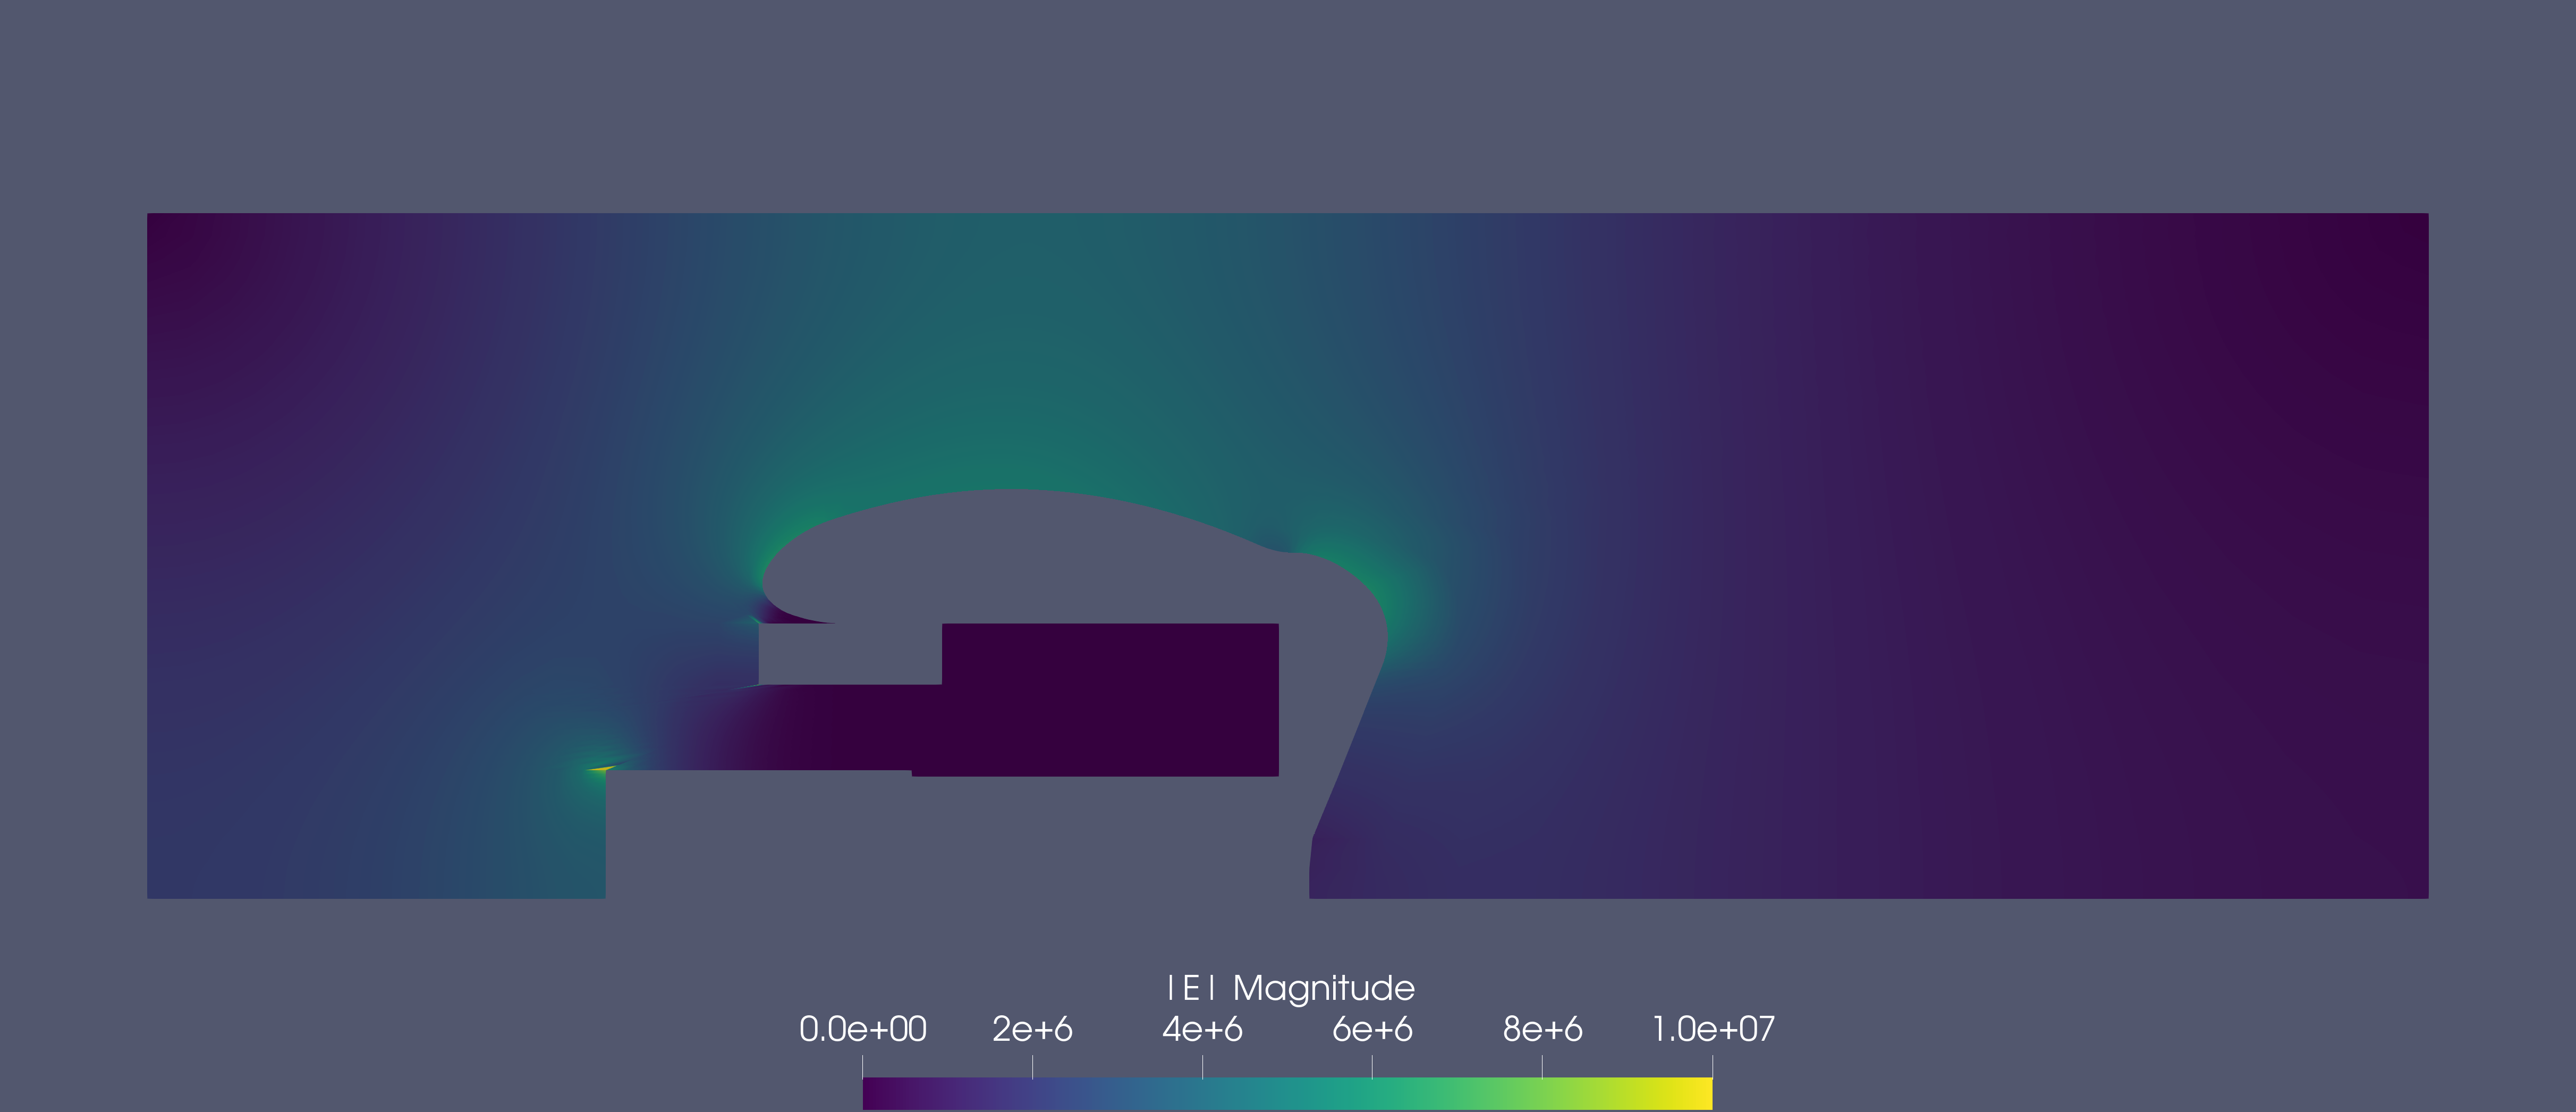
\includegraphics[width=\textwidth]{figures/200kV/png/cobyla_run11}
  \caption{Optimization result using COBYLA with $I=\{ 6, \dots, 11 \}$.}
  \label{fig:results_iga}
\end{figure}
\end{center}

In order to compare the results with the original geometry and simulation the optimized geometry was also imported and simulated in CST. The results indicate a clear improvement from the optimized geometry over the original one. This is in agreement with the numerical improvement observed in the context of IGA.

\begin{center}
\begin{figure}[H]
   \begin{subfigure}{0.45\textwidth}
      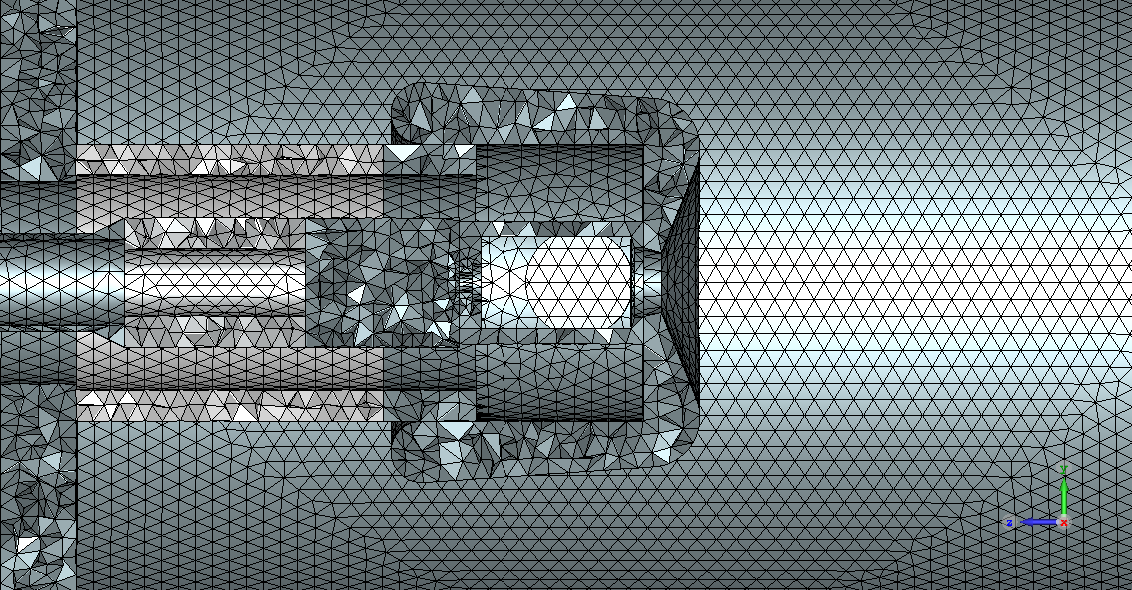
\includegraphics[width=\textwidth]{figures/200kV/cst/efield_orig_mesh}
   \end{subfigure}
   \begin{subfigure}{0.45\textwidth}
      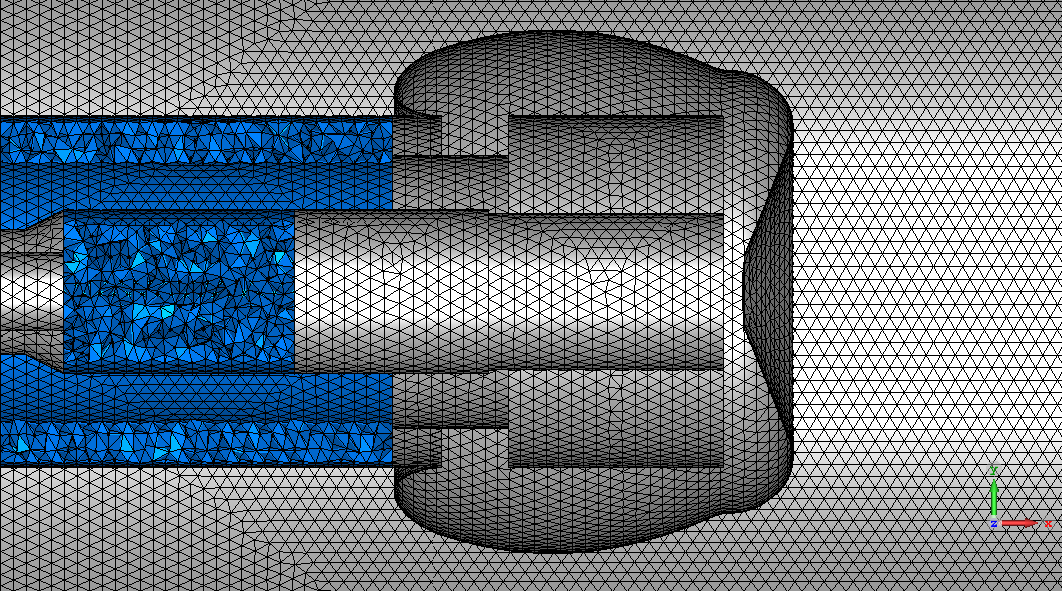
\includegraphics[width=\textwidth]{figures/200kV/cst/efield_mesh_new}
   \end{subfigure}
   \caption{Mesh of original and optimized geometry in CST.}
\end{figure}
\end{center}

\begin{center}
\begin{figure}[H]
   \begin{subfigure}{0.45\textwidth}
      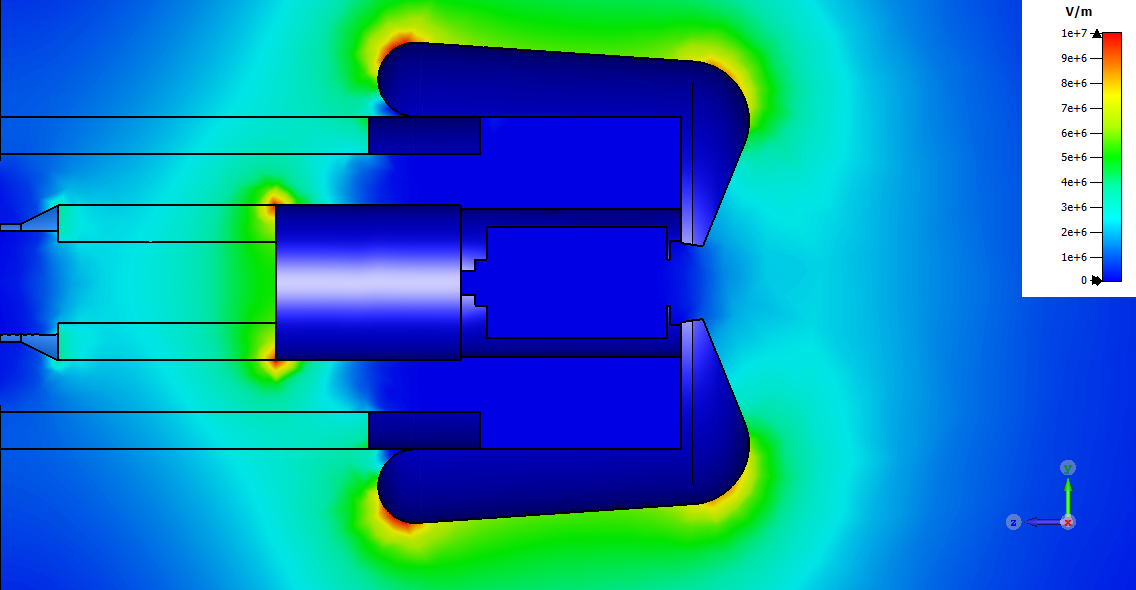
\includegraphics[width=\textwidth]{figures/200kV/cst/efield_orig}
   \end{subfigure}
   \begin{subfigure}{0.45\textwidth}
      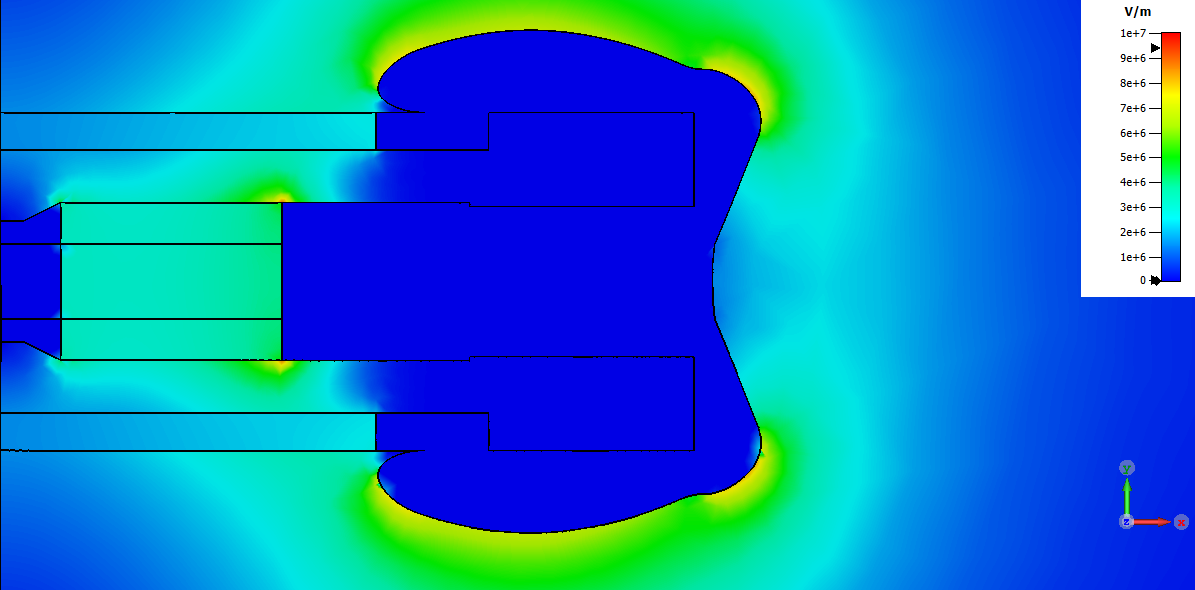
\includegraphics[width=\textwidth]{figures/200kV/cst/efield_insulator_new}
   \end{subfigure}
   \caption{Results of original and optimized geometry in CST.}
\end{figure}
\end{center}

\subsection{Questions}
\begin{itemize}
   \item should we consider the field strength in the insulator
   \item which part of the geometry should be optimized and why
   \item are the holes open during operation, should we consider them during optimization (3D simulation)
   \item what material does the dielectric strength of 10 MV/m refer to
\end{itemize}

\subsection{Astra}
In the future we may also optimize the electrode boundary next to the puck, i.~e.~patches 3, 4 and 5 to obtain optimal particle trajectories. The cost function will be computed using Astra.
The desired total bunch charge is $10$ pC with a beam current of $(20-100)\ \mu\mathrm{A}$, whereas a typical value would be $100$ fC. The bunch length is around $5$ ps with a normalized transversal emittance of $e_{x,y} \leq 1\ \mathrm{mm\: mrad}$. The desired energy resolution is $\frac{\Delta E}{E} \leq 10^{-4}$.
The tracking will be performed using individual bunches from a pulsed laser. The emission model may be derived from \cite{wagner}.
